\chapter{协议语义感知变异增强方法}

为了解决传统协议模糊测试工具对协议语义理解不足的问题，本文设计了一种大语言模型辅助的协议语义感知变异增强方法。该方法设计主要包括两个部分——\textbf{大模型智能体驱动的测试组件生成流水线}，以及适配生成组件的\textbf{两阶段变异策略}。

\section{方法概述}

图 \ref{fig:method_overview} 展示了该方法的整体概览。
该方法利用大语言模型的代码生成与语义理解能力，通过构建基于大模型智能体（LLM Agent）的自动化流水线，实现从协议规范解析到测试组件生成的端到端自动化流程。借助该流水线，可以针对新协议自动生成包括数据模型、变异器以及修复器，快速构建出具有协议语义感知能力的测试组件，显著降低了协议建模的人工成本。

进一步地，该方法还对现有的成熟模糊测试框架 Peach 进行了拓展与适配，设计了 LLMPeach 测试框架。该框架为大模型生成的测试组件提供了接口和检验器，并设计了两阶段变异策略，以充分利用生成组件的能力，同时不放弃传统变异器的带来的随机性，从而兼顾测试用例的多样性与语义合理性。

\begin{figure}[H]
\centering

\includegraphics[width=\textwidth]{source/method.pdf}
\bicaption{协议语义感知变异增强方法概览}{Overview of the Protocol Semantic-Aware Mutation Enhancement Method}
\label{fig:method_overview}
\end{figure}

\section{大模型智能体驱动的测试组件生成流水线}

图 \ref{fig:method_design} 展示了该流水线的整体设计。首先，系统通过检索增强生成（RAG）技术构建知识库，并引导大语言模型提取协议的报文类型。随后，针对每种报文类型，系统进一步引导模型进行字段建模，生成包含字段含义、取值约束及逻辑关联的结构化数据模型。最后，大语言模型基于数据模型构造出语义相关的变异器（Mutator）；结合协议的约束规则，构建自适应修复器（Fixer）以纠正因变异引入的语义违规行为。

\begin{figure}[H]
    \centering
    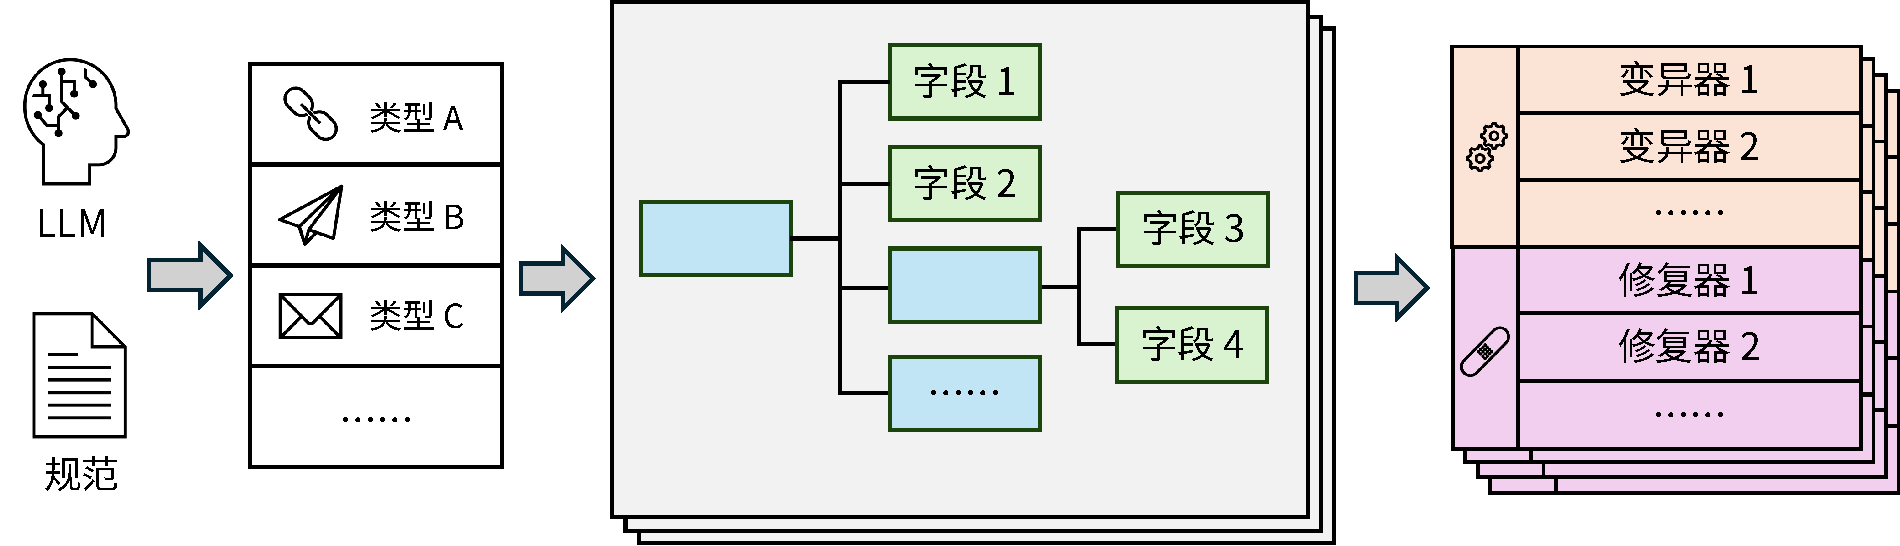
\includegraphics[width=\textwidth]{source/steps.pdf}
    \bicaption{大模型智能体驱动的测试组件生成流水线设计}{Design of the LLM Agent-Driven Test Component Generation Pipeline}
    \label{fig:method_design}
\end{figure}



为了高效地理解协议规范，系统中引入了检索增强生成\cite{lewis2020rag}（Retrieval-Augmented Generation, RAG）技术。RAG 技术允许大语言模型在生成过程中实时访问外部知识库——即目标协议的规范文档。通过将长篇幅的协议文档向量化并存储于检索器中，系统能够根据当前的解析需求，在知识库中进行检索，提取出协议规范文档中的相关段落，并将其作为上下文输入给模型。这种方式不仅解决了大语言模型在处理超长文档时的上下文窗口限制问题，还能够降低大模型产生“幻觉”的概率，确保生成的数据结构描述具有权威的文档支撑。

\subsection{报文类型提取}

``报文类型提取''是整个生成任务的第一步，其目标是识别出该协议中所有的报文类别。
图 \ref{fig:prompt_1} 展示了用于报文类型提取的提示词设计。其旨在驱动大语言模型智能体调用检索工具（如 RFC\_Search），在海量的文档文本中定位涉及报文格式定义的章节，并根据这些章节的内容，
忽略冗余的叙述性文字，仅抽取出协议报文的类型列表，并以特定的格式输出。

\begin{figure}[H]
\centering
\begin{tcolorbox}[
    before upper=\linespread{1.2}\selectfont
]
\bfsf{Task:} For <protocol> protocol, list ALL the packet types according to the RFC document.

Use the ``RFC\_Search" tool to look up the relevant sections in the RFC.

Return the list as a comma-separated string.
ONLY output the types, nothing else.

\textit{[Example]}

\prule

\bfsf{Tool:} RFC\_Search
\end{tcolorbox}
\bicaption{报文类型提取的提示词设计}{Prompt Design for Packet Type Extraction}
\label{fig:prompt_1}
\end{figure}

提取出的报文类型列表将作为元数据存储于系统的全局状态中，为后续针对每种具体报文进行建模提供明确的目标。

\subsection{数据模型生成、检验与修复}

在获取了协议的报文类型清单后，流水线进入第二阶段——针对每种特定报文构建精细化的 Peach 数据模型。
此步骤是整个生成流水线的关键，因为数据模型的质量将直接影响后续变异器和修复器的效果。
大语言模型需要深入理解每个字段的基本含义（位宽、偏移、类型）以及语义关联（校验和、长度依赖、状态标志），并将这些信息以 Peach 数据模型的 XML 格式进行建模。

为了确保生成的数据模型的准确性与实用性，设计方案并未采用一次性的直接生成策略，而是构建了一个“生成—验证—修复”的闭环流水线，以应对大语言模型在生成结构化数据时可能出现的格式错误、语义误解或遗漏问题。

图 \ref{fig:data_model} 展示了数据模型生成与检验的流程设计。
大语言模型首先进行数据模型的生成，随后通过检验脚本对生成的数据模型进行验证。若验证失败，系统引导模型修复错误，并重新生成数据模型。该流程将持续迭代，直到生成的模型通过所有检验项为止。
\begin{figure}[H]
    \centering
    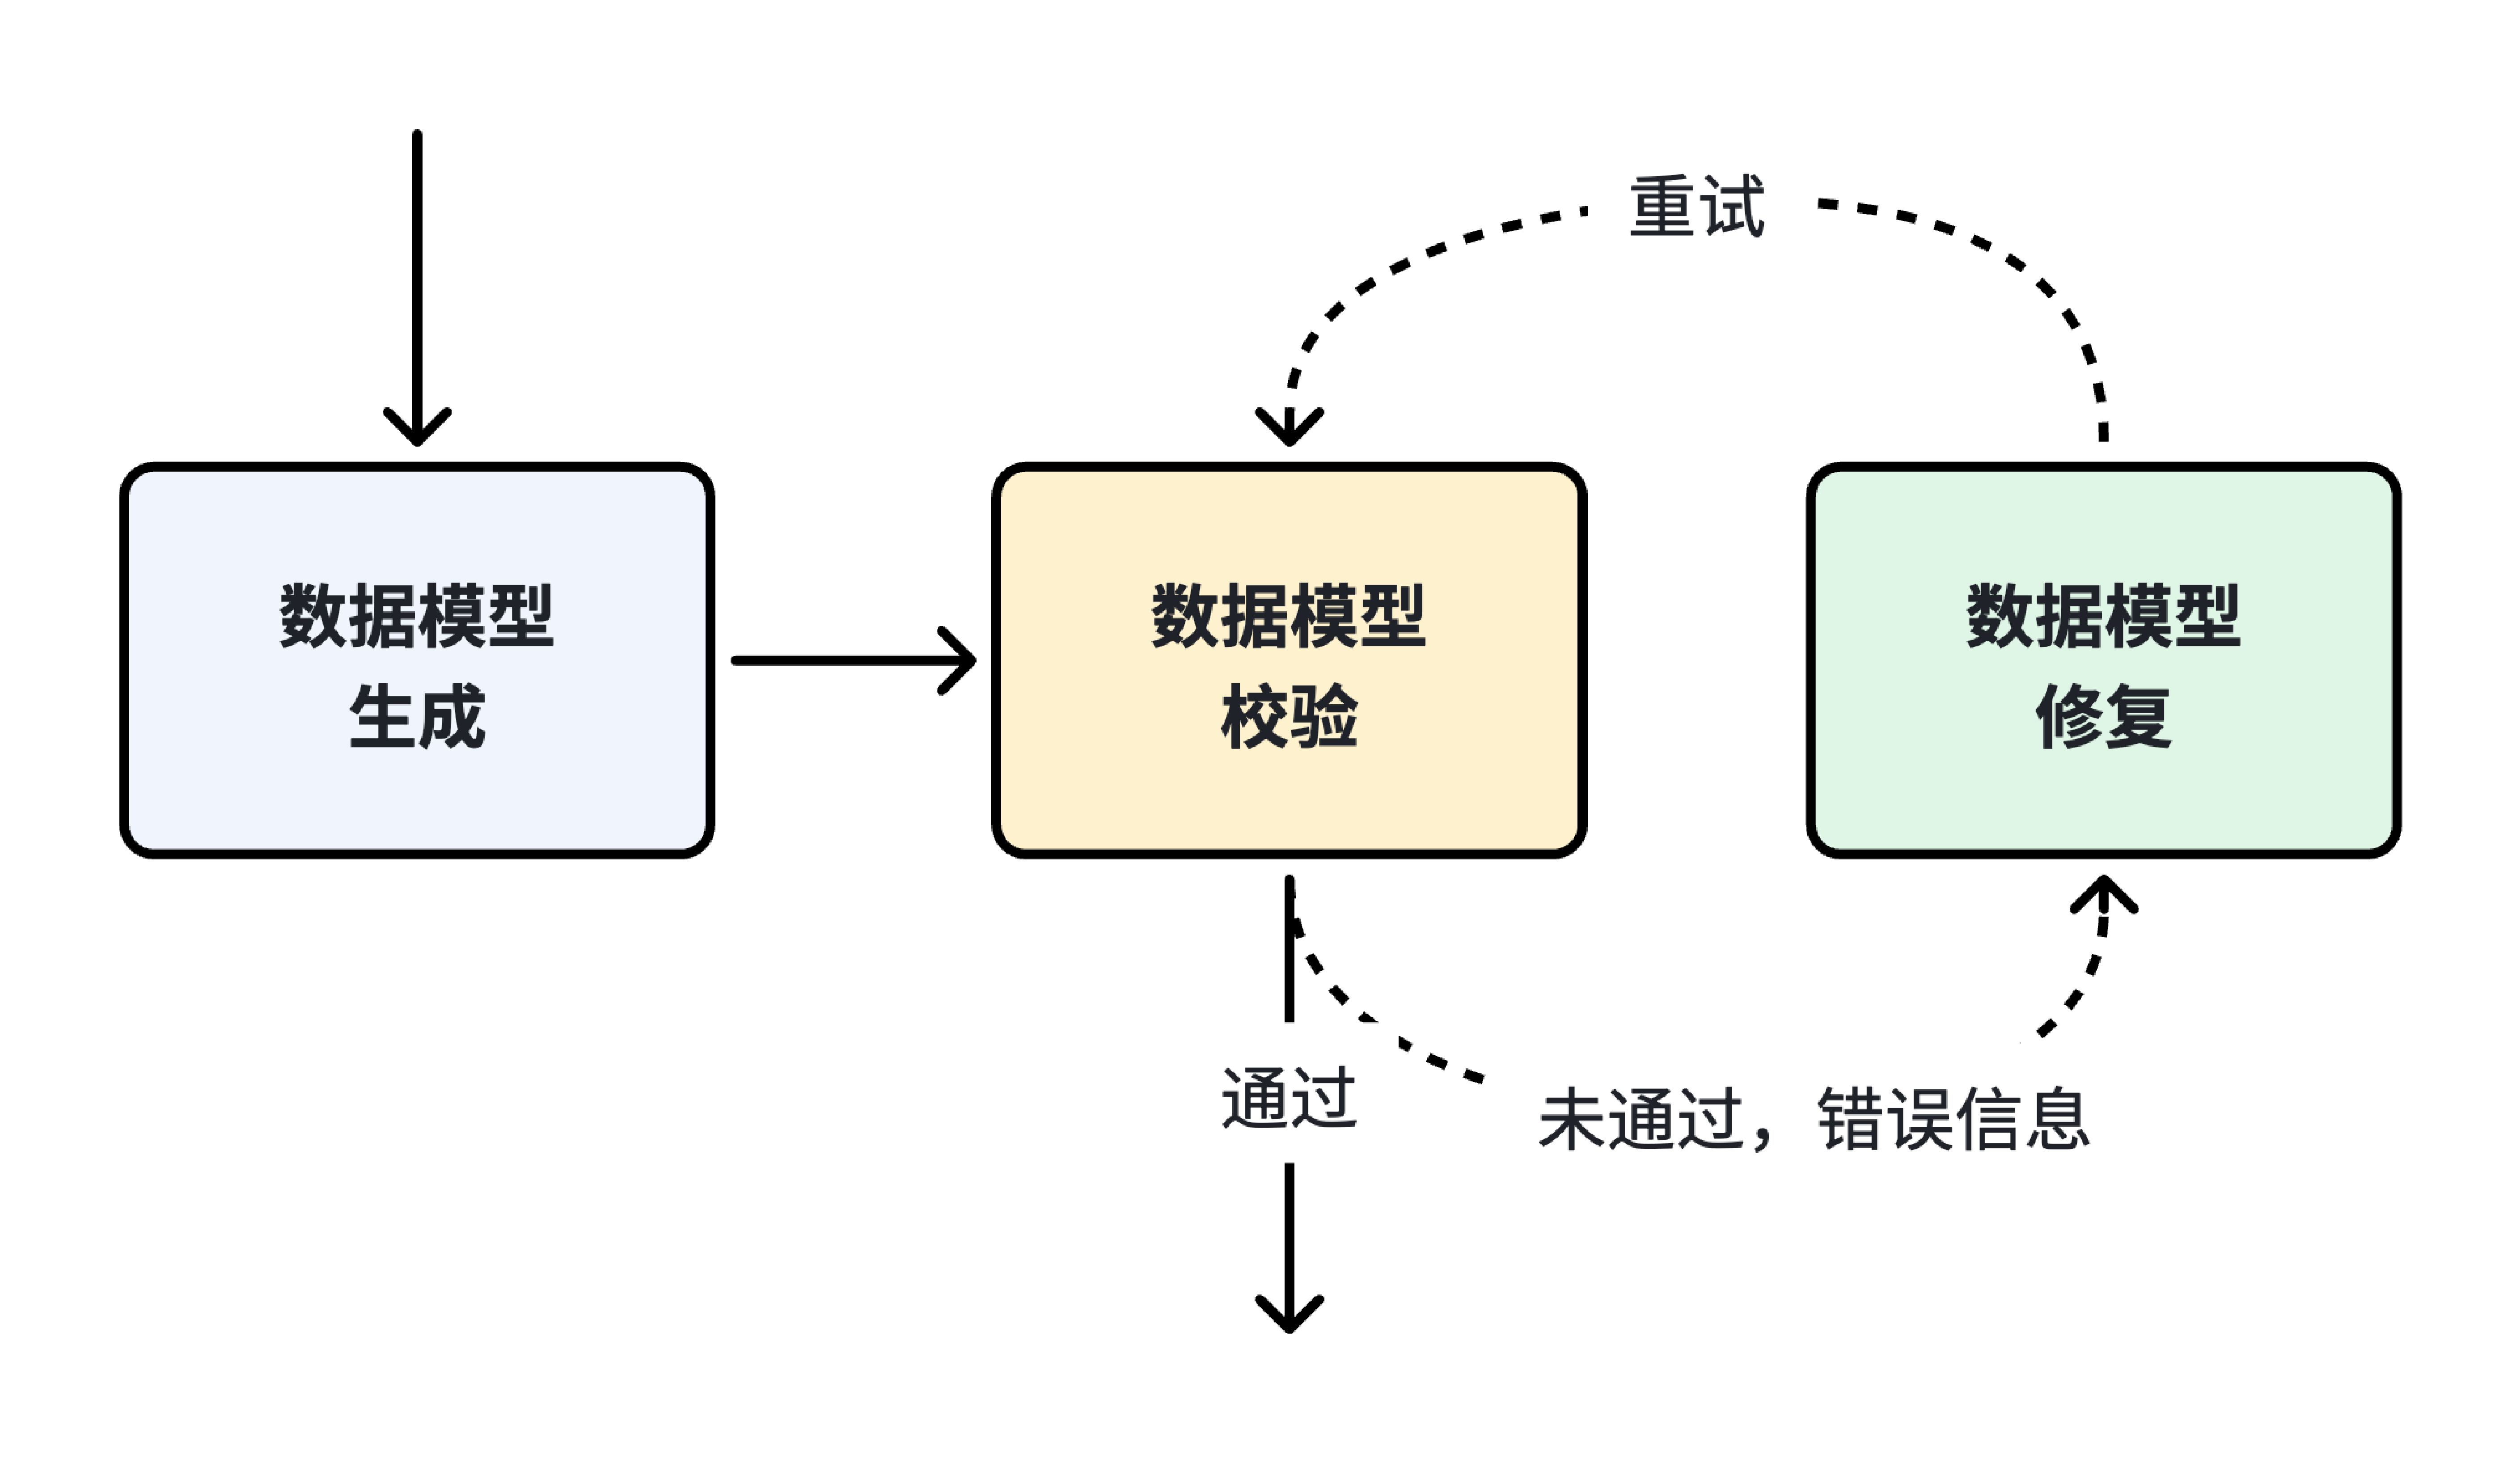
\includegraphics[width=0.6\textwidth]{source/dm.pdf}
    \bicaption{数据模型生成与检验流程}{Data Model Generation and Validation Process}
    \label{fig:data_model}
\end{figure}

\textbf{数据模型生成}。如图 \ref{fig:prompt_2} 所示，这一阶段以先前提取的报文类型列表为输入，并结合协议规范文档中对报文格式与语义约束的描述，要求大模型对各类报文的结构进行细粒度建模。
在提示词中，明确规定了模型需要遵循的建模原则，包括如何利用 XML 元素刻画字段类型、长度、取值范围以及字段间的依赖关系（如长度字段与数据字段之间的关联）。
同时，通过补充示例与操作提示（如 Relation、Optional 和 Block 等关键机制的使用方式），这些操作提示促使模型能够主动运用这些机制，进一步约束生成结果的表达形式与完整性。
此外，该提示词还包含了从 Peach 的说明文档中提取的数据模型中相关数据类型的说明性文本，以帮助模型更准确地理解 Peach 数据模型的语义要求，从而生成符合规范的数据模型。


\begin{figure}[H]
\centering
\begin{tcolorbox}[
    before upper=\linespread{1.2}\selectfont
]
\bfsf{Task: }Using the packet types we just identified (<packet\_types>), generate a Peach Pit file defining the precise structure of each packet for <proto>. 

Model the structure as detail as possible.

\textit{[Example]}

Hint: 

1. Read the usage of each XML element in ``peach.txt" to understand how to define the structure for each packet type.

2. \textit{Other Hints...}

\prule

\bfsf{Tool:} RFC\_Search, Write\_File, Read\_File
\end{tcolorbox}

\bicaption{数据模型生成的提示词设计}{Prompt Design for Data Model Generation}
\label{fig:prompt_2}
\end{figure}

\textbf{数据模型检验}。为了尽可能提升生成的数据模型的质量，对数据模型进行检验是必不可少的环节。
大模型生成的数据模型中，通常可能出现以下几类问题：1）数据类型错误，如使用了Peach不支持的数据类型；2）字段定义错误，如字段的位宽、偏移或取值范围与协议规范不符；3）依赖关系错误，如长度字段未正确关联到数据字段，或校验字段未正确关联到被校验的数据字段等。4）结构错误，如缺失必要的字段或包含冗余字段等。5）过度简化，如未能充分利用 Peach 的机制来表达协议的复杂语义关系，导致生成的数据模型过于简化，无法准确反映协议的实际结构和约束。

针对这些潜在问题，此阶段引入了数据模型检验器，以自动化地检测生成的数据模型是否存在上述问题。
检验器会将预先准备的大量该协议的合法数据包作为测试输入，利用生成的数据模型进行解析，然后不经任何修改地将解析结果重新输出。通过比较输入与输出数据包的结构和内容是否一致，可以揭示生成的数据模型在字段定义、长度约束、依赖关系等方面是否存在错误或不完整之处。若检验失败，系统会将具体的错误信息连同解析日志一同输出。

\textbf{数据模型修复}。当检验阶段检测到生成的数据模型存在问题时，系统会进一步引导大语言模型对数据模型进行自动修复。
图 \ref{fig:prompt_3} 展示了数据模型修复的提示词设计。该提示词要求模型首先分析检验日志，定位数据模型中的具体错误（如字段解析失败、长度不匹配等），并输出清晰的错误解释。随后，模型需要根据错误信息对原有的数据模型进行针对性的修改，以修正这些问题。需要强调的是，在修复过程中，大模型被禁止简化数据模型的结构，避免其以过度简化的方式来规避问题，而是需要在保持数据模型完整性的前提下进行修复，以确保最终生成的数据模型能够准确反映协议的实际结构和约束。

\begin{figure}[H]
\centering
\begin{tcolorbox}[
    before upper=\linespread{1.2}\selectfont
]
\bfsf{Task: } We ran a verification test against the generated datamodel, which used the Peach Pit file to parse packets and check if the fields were correctly extracted. 
The test failed, indicating there are issues with the datamodel.

Here is the test output:
\textit{[Validation Output]}

You need to:

\begin{enumerate}
    \item Read EACH test log file in <test\_log\_directory> to identify the specific issues with the datamodel. Look for parsing errors, mismatched fields, or any indications of what part of the datamodel is incorrect.
    \item For each identified issue, output a clear explanation of what the problem is and which part of the datamodel it relates to.
    \item Modify the Peach Pit file to fix the identified issues.
\end{enumerate}

\textbf{CRITICAL}: Simplifying the DataModel is NOT allowed.

\prule

\bfsf{Tool:} Read\_File, Write\_File
\end{tcolorbox}
\bicaption{数据模型修复的提示词设计}{Prompt Design for Data Model Repair}
\label{fig:prompt_3}
\end{figure}

\subsection{变异器的生成、检验与修复}
在本阶段中，将进行变异器（Mutator）的构建。变异器决定了模糊测试工具如何在遵循协议基本语义的前提下，探索目标程序的边界条件与逻辑漏洞，被视为模糊测试的核心组件之一。

为了实现更深层、更具语义感知的测试，本方法不再依赖 Peach 框架内置的通用变异算子，而是利用大语言模型针对协议的每一个字段生成定制化的 C\# 变异逻辑。这些定制变异器能够理解字段的业务逻辑，例如生成常见值、边界值等。

如图 \ref{fig:mutator_process} 所示，与数据模型的生成流程不同，变异器在生成时采取了并行化的设计思路，即针对每个字段的变异器生成任务可以同时进行，以提升整体效率。另一方面，这样处理也能够减少每个变异器生成时的上下文复杂度，使得大语言模型能够更专注于单一字段的语义特征，从而生成更精准的变异逻辑。
同样，为了确保生成的代码能够正常编译并符合 Peach 的接口规范，该过程依然遵循“生成—验证—修复”的循环逻辑。

\begin{figure}[H]
    \centering
    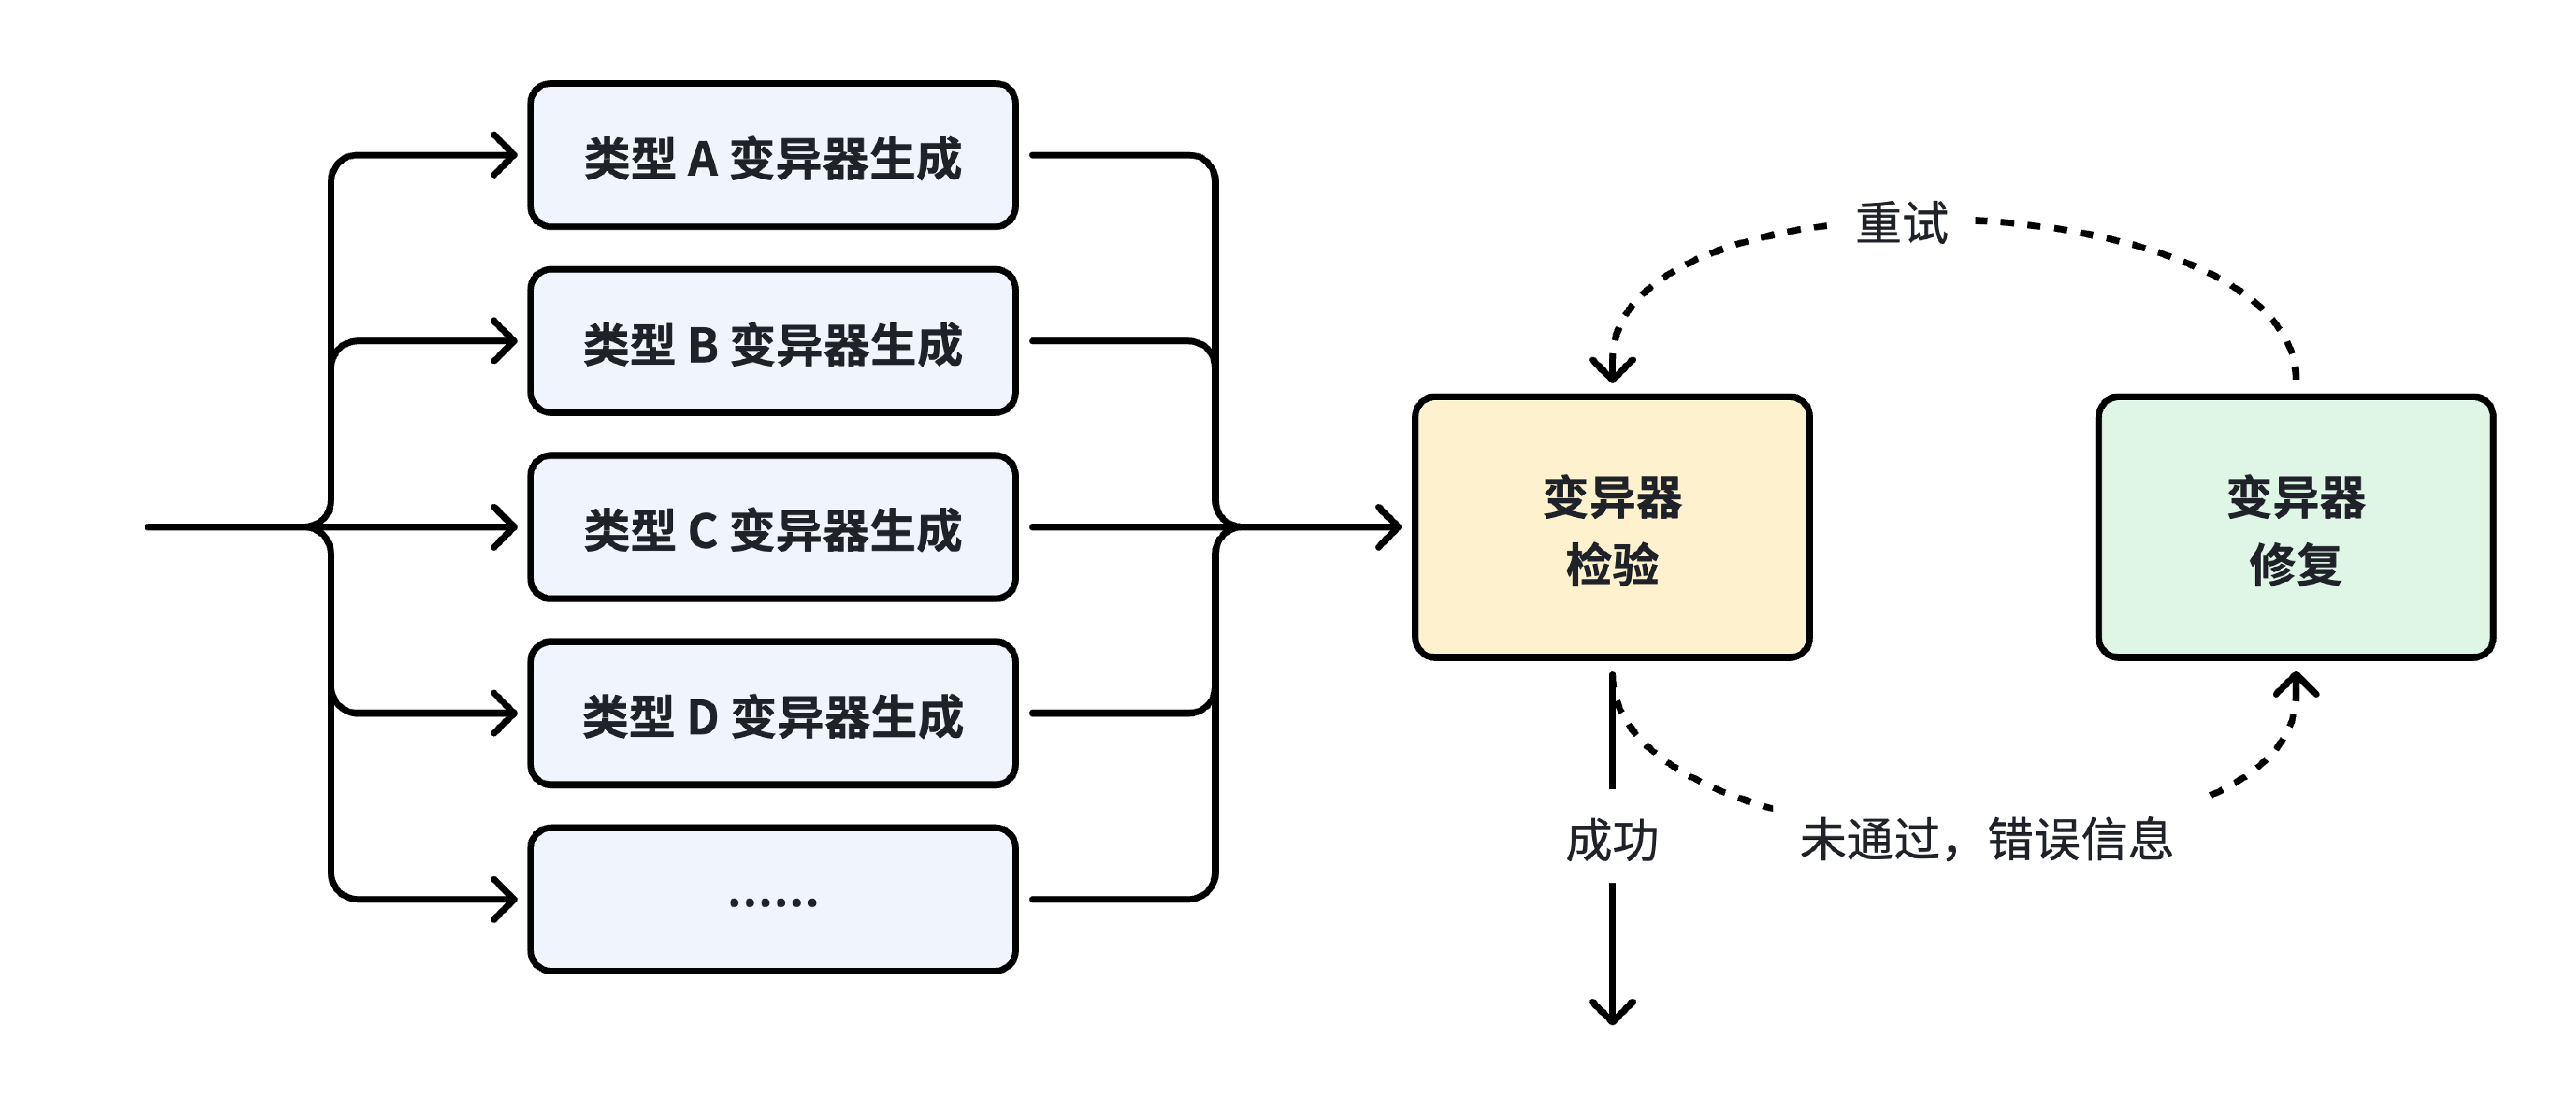
\includegraphics[width=\textwidth]{source/mutator.pdf}
    \bicaption{变异器生成、检验与修复流程}{Mutator Generation, Validation and Repair Process}
    \label{fig:mutator_process}
\end{figure}

\textbf{变异器生成}。如图 \ref{fig:prompt_mutator_gen} 所示，在此阶段，对于每种协议包类型，大语言模型需要根据规范文档和先前生成的数据模型，先列出该消息包类型中包含的全部字段。对于每个字段，大模型需要对其分类处理——对于取值固定的字段，不生成任何变异逻辑；而对于可变字段，则根据其结构特征（如是否可选、是否可重复）生成对应的结构性操作类（例如 Add、Remove、Repeat）。

对于可变字段的设计是变异器生成的核心。提示词明确规定需要围绕字段的局部语义属性构建多维度的变异策略，具体涵盖八类语义范畴：A)规范形式（Canonical form），用于生成符合标准语义的推荐取值；B)边界值（Boundaries），用于探索字段取值空间的上下界及临界点；C)等价类替代（Equivalence-class alternatives），通过替换为语义上有效但结构不同的值以触发潜在分支；D)合法位域/枚举/范围（Allowed bitfield/enum/range），适用于具有明确取值集合的字段；E)编码形态变体（Encoding-shape variant），例如不同编码方式或长度表示形式的切换；F)填充与对齐（Padding/alignment），用于测试实现中对内存对齐或填充字节的处理逻辑；G)前缀/后缀扰动（Prefix/Suffix），通过在字段前后添加特定模式以探测解析器的鲁棒性；H)随机合法混合（Random valid mix），用于生成组合型输入以提升测试多样性。

总的来说，变异器生成阶段以协议字段为核心，将其按可变性与语义特征进行系统化拆解，并围绕多维语义范畴设计针对性的变异策略。通过结合结构性操作与语义驱动的取值生成方法，不仅能够覆盖常规与边界输入，还能探索多样化且具有潜在触发效果的测试数据，从而提升协议实现的测试深度与缺陷发现能力。

\begin{figure}[H]
\centering
\begin{tcolorbox}[
  before upper=\linespread{1.2}\selectfont
]
\bfsf{Task: } List ALL fields for the <protocol> <packet\_type> packet.

For EACH field <field\_name> in the <protocol> <packet\_type> packet:
\begin{enumerate}[noitemsep,leftmargin=*]
    \item \textbf{Fixed value?} If the field is fixed, do not generate any mutator functions.

    \item \textbf{Otherwise (the field is mutable):}
    \begin{enumerate}[noitemsep]
        \item If the field is optional, implement:
        \begin{itemize}[noitemsep,label={},leftmargin=*]
            \item \texttt{class <PROTO><PacketType>Add<FiledName>}
            \item \texttt{class <PROTO><PacketType>Remove<FiledName>}
        \end{itemize}

        \item If the field may appear multiple times, also implement:
        \begin{itemize}[noitemsep,label={},leftmargin=*]
            \item \texttt{class <PROTO><PacketType>Repeat<FiledName>}
        \end{itemize}

        \item \textbf{Mutate.} Design semantic-aware mutators for this field by covering the following field-local semantic categories:
        
            \begin{tabular}{ll}
A. Canonical form & B. Boundaries \\ 
C. Equivalence-class alternatives &
D. Allowed bitfield/enum/range \\ 
E. Encoding-shape variant & F. Padding/alignment \\
G. prefix/suffix & H. Random valid mix \\
\end{tabular}

        Add randomized perturbations mixing shallow and deep changes to preserve long-term diversity and avoid collapse into a single pattern.

        \begin{itemize}[noitemsep, label={},leftmargin=*]
            \item \texttt{class <PROTO><PacketType>Mutate<FiledName>}
        \end{itemize}
    \end{enumerate}
\end{enumerate}
Write in C\# 5.0. Inherit from <class LLMMutator> in the LLMPeach SDK.

\textit{[Example]}

\prule

\bfsf{Tool:} RFC\_Search, Write\_File, Read\_File, Build\_DotNet\_DLL, Search\_Class
\end{tcolorbox}
\bicaption{变异器生成的提示词设计}{Prompt Design for Mutator Generation}
\label{fig:prompt_mutator_gen}
\end{figure}

在变异器的生成过程中，大模型智能体可以利用多种辅助工具（Tool）提升生成质量。其中，\texttt{RFC\_Search} 用于检索协议规范中的字段定义与约束信息，为变异逻辑提供权威的语义依据；
\texttt{Read\_File} 与 \texttt{Write\_File} 分别用于读取模板代码与输出生成结果；\texttt{Build\_DotNet\_DLL} 用于对生成的 C\# 代码进行编译验证。特别地，\texttt{Search\_Class} 工具可从 LLMPeach SDK 已编译的库文件中检索指定类，并展示其方法接口与继承结构，从而帮助模型准确理解库中相关类（如 \texttt{LLMMutator}）的使用方式，减少接口误用带来的生成错误。通过上述工具的协同配合，可以有效提升变异器生成结果的正确性与工程可用性。

\textbf{变异器检验}。变异器的检验与数据模型的检验有所不同。检验脚本会在合法的测试输入上运行生成的变异器，并检查其变异的结果。每个变异器都将被测试数百次，以减少随机性的影响。对于每一个被测试的变异器，如果其变异途中发生了错误，或在100轮测试中未能成功生成任何一个合法的变异结果，则认为该变异器存在问题，需要进入修复流程。

\textbf{变异器修复}。如图 \ref{fig:prompt_mutator_repair} 所示，这一阶段以变异器验证测试的错误输出为输入，指导大语言模型对存在缺陷的变异器进行定位与修复。提示词要求模型根据报错信息分析异常原因，读取对应的 C\# 源文件，并针对关键逻辑中可能存在的空值访问、越界操作或不合理处理进行修正。在完成修改后，通过 \texttt{Write\_File} 更新代码，并利用 \texttt{Build\_DotNet\_DLL} 进行重新编译验证，从而确保修复后的变异器在语法与运行层面不会触发异常。

\begin{figure}[H]
\centering
\begin{tcolorbox}[
  before upper=\linespread{1.2}\selectfont
]
\bfsf{Task: } We ran a verification test against the generated mutators. The test failed with an ERROR for the mutator <mutator\_name>.

Here is the test error output for this mutator:

\textit{[Validation Output]}

The test logs indicate there are issues with the generated C\# code for <mutator\_name>. 

You need to:
\begin{enumerate}[noitemsep]
    \item Find the C\# file containing the <mutator\_name> class.
    \item Analyze the traceback and error message to understand the logic flaw or runtime exception.
    \item Use the ``Read\_File" tool to read the corresponding mutator file.
    \item Fix the bug in the C\# code. Make sure to handle potential nulls, index out of bounds, etc., that might occur during `PerformMutation'.
    \item Use the ``Write\_File" tool to update the file with the fix.
    \item Use the ``Build\_DotNet\_DLL" tool to recompile the mutators and ensure there are no syntax errors.
\end{enumerate}

Be thorough and ensure the C\# code will successfully compile.

\prule

\bfsf{Tool:} Read\_File, Write\_File, Build\_DotNet\_DLL
\end{tcolorbox}
\bicaption{变异器修复的提示词设计}{Prompt Design for Mutator Repair}
\label{fig:prompt_mutator_repair}
\end{figure}

\subsection{修复器的生成、检验与修复}

在此阶段，将完成修复器（Fixer）的构建。修复器可以修复在变异过程中可能引入的语义违规行为，以确保生成的测试用例在保持多样性的同时，仍然能够满足协议的基本语义约束，从而提高测试效率和有效性。

图 \ref{fig:fixer_process} 展示了修复器的生成、检验与修复流程设计。与变异器类似，修复器的生成也遵循“生成—验证—修复”的循环逻辑，以提高其功能的正确性与实用性。
此流程主要分为约束提取、修复器生成、约束修复测试生成、修复器检验与修复器修复五个模块。首先，大模型会提取该协议规范中的约束，随后，针对这些约束，并行地生成修复器代码和约束修复测试用例。接着，检验模块会运行修复器并检查其是否能够成功修复变异引入的语义违规行为。若检验失败，系统会引导模型分析失败原因并对修复器进行针对性的修正，直到生成的修复器能够通过所有检验项为止。

值得注意的是，虽然针对的是相同的约束，修复器的生成和约束修复测试的生成是分别进行的。在进行约束修复测试的生成时，模型没有生成修复器的记忆，提示词也不允许模型查看对应约束的修复器代码，以确保测试用例的独立性和有效性。

\begin{figure}[H]
    \centering
    \includegraphics[width=\textwidth]{source/fixer.pdf}
    \bicaption{修复器生成、检验与修复流程}{Fixer Generation, Validation and Repair Process}
    \label{fig:fixer_process}
\end{figure}

\textbf{约束提取}。如图 \ref{fig:prompt_constraint_extraction} 所示，这一阶段以协议规范文档为输入，要求大语言模型从 RFC 中系统性地提取所有与客户端到服务器请求报文相关的格式约束。提示词引导模型重点关注规范中以强制性语言（如 MUST、MUST NOT、SHALL 等）描述的规则，并将其整理输出，为后续修复器的生成与验证做好准备。

\begin{figure}[H]
\centering
\begin{tcolorbox}[
    before upper=\linespread{1.2}\selectfont
]
\bfsf{Task: } Extract all constraints related to request (client to server) message format from the <proto> RFC.
For example, in MQTT there are the following constraints:
\begin{itemize}[noitemsep, label={-}, leftmargin=*]
    \item[-] [MQTT-2.2.1-2] A PUBLISH packet MUST NOT contain a Packet Identifier if its QoS value is set to 0.
    \item[-] [MQTT-3.1.2-11] If the Will Flag is set to 0, then the Will QoS MUST be set to 0 (0x00).
    \item[-] ...
\end{itemize}

\prule

\bfsf{Tool:} RFC\_Search
\end{tcolorbox}
\bicaption{约束提取的提示词设计}{Prompt Design for Constraint Extraction}
\label{fig:prompt_constraint_extraction}
\end{figure}

\textbf{修复器生成}。如图 \ref{fig:prompt_fixer_gen} 所示，该阶段围绕已提取的协议约束，要求大语言模型为每条约束构建对应的修复逻辑，从而对不符合规范的报文进行就地调整。

\begin{figure}[H]
\centering
\begin{tcolorbox}[
    before upper=\linespread{1.5}\selectfont
]
\bfsf{Task: } For <protocol>, write fixer functions for EACH constraint below.

Write in C\# 5.0.
File: <fixer\_file\_name>.cs

\textit{[Example]}

The input is a single packet. Fix in place.

HINTS

\begin{itemize}[noitemsep, label={-}, leftmargin=*]

\item Change a field value: \texttt{obj.SetValue(new Variant(...))};

\item Remove a field: \texttt{obj.parent.Remove(obj)};

\item Make `Optional' field exist: \texttt{obj.SetValue(new Variant(...))} on its child field(s) with valid value(s).
\end{itemize}


Constraints for this task:
<constraint\_list>

You must ensure there are NO syntax errors and the code compiles successfully.

\prule

\bfsf{Tool:} Read\_File, Write\_File, Build\_DotNet\_DLL, Search\_Class
\end{tcolorbox}
\bicaption{修复器生成的提示词设计}{Prompt Design for Fixer Generation}
\label{fig:prompt_fixer_gen}
\end{figure}

\textbf{约束修复测试生成}。如图 \ref{fig:prompt_fixer_test} ，该提示词用于指导大语言模型基于协议约束自动生成对应的测试用例，以验证每个修复器（Fixer）的正确性。其核心目标是：针对输入的每一条约束，首先构造一份违反对应约束的报文数据；接着调用待测试的 Fixer 函数对报文进行修复；最后通过断言验证修复结果是否恢复到满足约束的状态。

\begin{figure}[H]
\centering
\begin{tcolorbox}[
  before upper=\linespread{1.2}\selectfont
]
\bfsf{Task: } For <protocol>, write NUnit test functions for validating EACH fixer constraint below.

\textit{[Constraints]}


Write in C\# 5.0.

\textit{[Example]}

{Test Workflow:}
\begin{enumerate}[noitemsep]
    \item Construct packet data that violates the constraint.
    \item Invoke the corresponding Fixer function.
    \item Assert that the Fixer restores the constraint.
\end{enumerate}

\textbf{IMPORTANT:}
\begin{itemize}[noitemsep]
    \item Ensure NO syntax errors and successful compilation.
    \item Treat Fixers as a black box; do NOT inspect their implementation.
\end{itemize}

\prule

\bfsf{Tool:} Read\_File, Write\_File, Build\_DotNet\_DLL
\end{tcolorbox}
\bicaption{约束修复测试生成的提示词设计}{Prompt Design for Constraint Fix Test Generation}
\label{fig:prompt_fixer_test}
\end{figure}

\textbf{修复器检验}。修复器的检验主要通过运行前面生成的约束修复测试来完成。每个修复器都将对应一个或多个测试用例，这些测试用例会构造出违反特定约束的输入数据，并调用修复器进行修正。检验脚本会检查修复后的结果是否满足原有的约束条件，从而验证修复器的功能正确性。如果某个修复器未能通过其对应的测试用例，则认为该修复器存在缺陷，需要进入修复流程。

\textbf{修复器修复}。当修复器检验失败时，系统会引导大语言模型对存在缺陷的修复器进行定位与修正。
如图 \ref{fig:prompt_fixer_repair} 所示，
这个过程与变异器的修复类似。大模型需要分析测试失败的具体原因，读取对应的 C\# 源文件，并针对关键逻辑中可能存在的问题进行修正。在完成修改后，更新代码，并重新编译验证，直到修复器能够通过所有相关测试用例为止。

\begin{figure}[H]
\centering
\begin{tcolorbox}[
  before upper=\linespread{1.2}\selectfont
]
\bfsf{Task: } We ran a verification test against the generated fixers. The test failed with an ERROR for the fixer <fixer\_name>.

Here is the test error output for this fixer:

\textit{[Validation Output]}

The test logs indicate there are issues with the generated C\# code for <fixer\_name>. 

\textit{[Repair Steps]}

\prule

\bfsf{Tool:} Read\_File, Write\_File, Build\_DotNet\_DLL
\end{tcolorbox}
\bicaption{修复器修复的提示词设计}{Prompt Design for Fixer Repair}
\label{fig:prompt_fixer_repair}
\end{figure}

\section{两阶段变异策略}

为了充分发挥大模型生成的变异器和修复器的能力，本方法设计了一套两阶段的变异策略。图 \ref{fig:mutation_strategy} 展示了该策略的基本流程。

\begin{figure}[H]
    \centering
    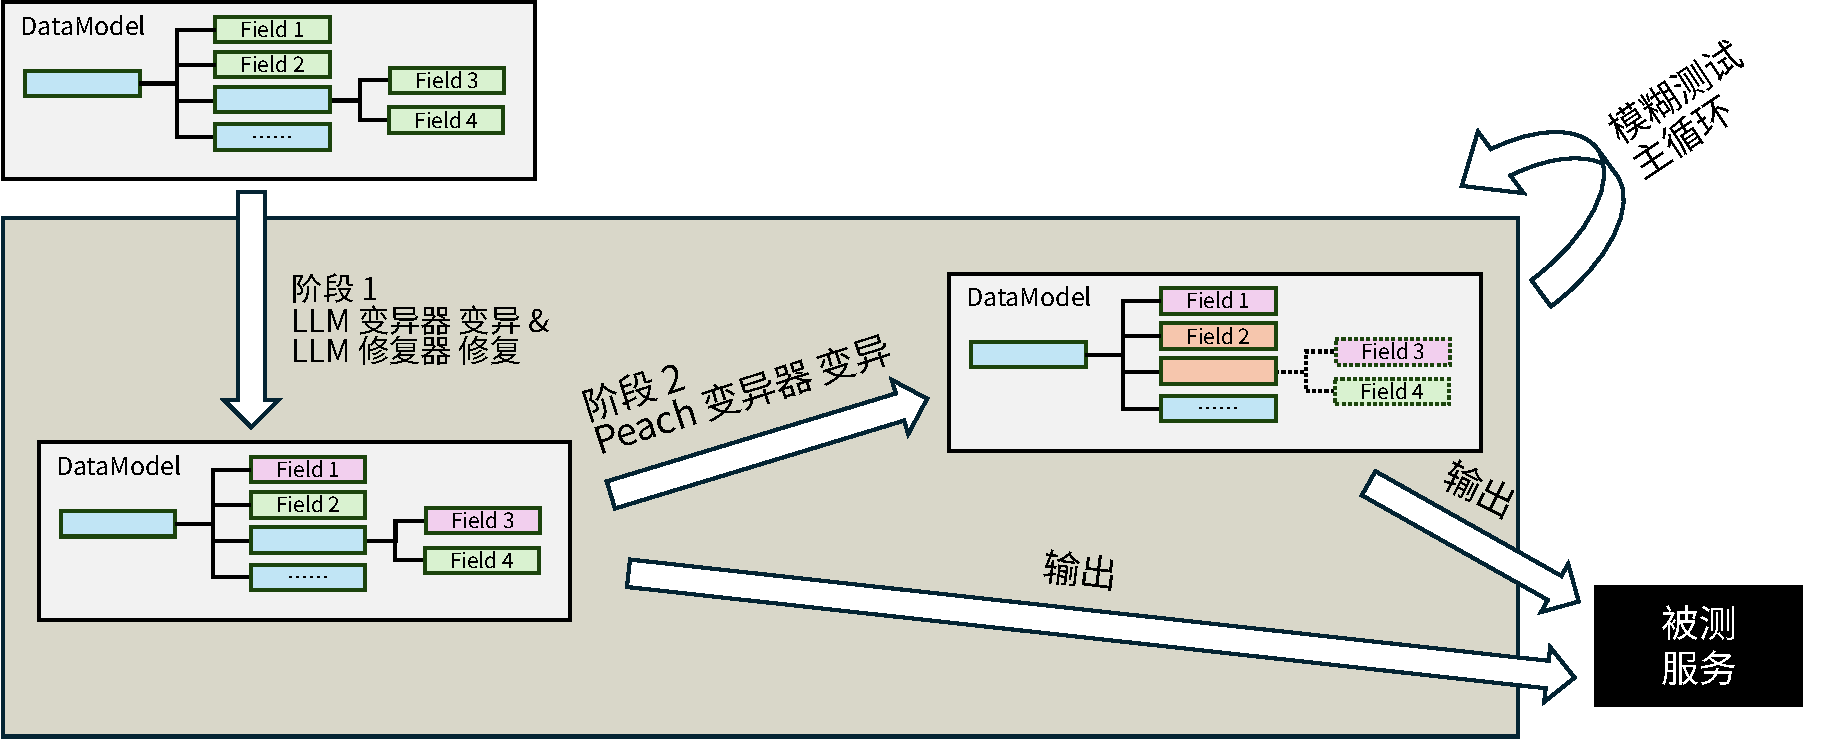
\includegraphics[width=\textwidth]{source/twophase.pdf}
    \bicaption{两阶段变异策略设计}{Design of the Two-Stage Mutation Strategy}
    \label{fig:mutation_strategy}
\end{figure}

图 \ref{fig:two_phase_algorithm} 展示了两阶段变异策略算法。
该策略将变异过程划分为两个阶段，以兼顾输入语义有效性与测试扰动强度。第一阶段采用大语言模型（LLM）生成的变异器，作用于具备语义结构的字段，对输入进行协议语义相关的变异，在扩展输入空间的同时尽可能维持协议约束与上下文一致性。此外，引入 修复器 对变异结果进行约束修正，以确保生成的数据满足基本语法与语义合法性，从而提高有效测试样本的比例。

第二阶段使用传统变异器（如边界值修改、随机比特翻转、枚举扰动等）对所有候选字段进行进一步变异。该阶段不再强调语义保持，而是通过更具破坏性的操作引入异常输入，以触发潜在的边界错误、解析异常或状态机缺陷，从而增强测试的探索能力和覆盖范围。

在每个阶段中，针对单个元素的变异次数并非固定，而是从区间 $[1, k]$ 中通过加权随机分布进行采样，其中较小的变异次数具有更高概率。这种设计避免了过度变异导致的语义完全破坏，同时允许一定概率的多次连续变异，以探索更远离初始输入的状态空间，在保持数据包合法和扩大探索范围之间取得平衡。

\begin{figure}[H]
\begin{minipage}{\textwidth}
\begin{algorithm}[H]
\caption{两阶段变异策略}
\begin{algorithmic}[1]
\fontsize{10pt}{8pt}\selectfont
\Require 动作 $a$，变异集合 $M$，最大变异次数 $k$，LLM 变异器集合 $\mathcal{M}_{LLM}$
\Ensure 变异后的数据模型 $D$

\State $D \gets a.outputData$

\State $S_1 \gets \{ e \in M \mid e.Mutators \cap \mathcal{M}_{LLM} \neq \emptyset \}$ 
\ForAll{$e \in S_1$} \Comment{阶段一：LLM 变异}
    \State $n \sim \mathcal{W}(1,k)$
    \For{$i = 1$ to $n$}
        \State $m$ $\gets$ $RandPick(e.Mutators)$ \Comment{随机选择一个 LLM 变异器}
    \EndFor
\EndFor
\State $D.fixup()$ \Comment{应用修复器修正语义违规}
\State $a.Output(D)$ \Comment{输出阶段一产物}

\ForAll{$e \in M$} \Comment{阶段二：非LLM变异}
    \State $n \sim \mathcal{W}(1,k)$
    \For{$i = 1$ to $n$}
        \State $m$ $\gets$ $RandPick(e.Mutators \setminus \mathcal{M}_{LLM})$ \Comment{随机选择一个非LLM变异器}
    \EndFor
\EndFor

\State $a.Output(D)$ \Comment{输出阶段二产物}

\end{algorithmic}
\end{algorithm}
\end{minipage}

\bicaption{两阶段变异策略算法}{Algorithm of the Two-Stage Mutation Strategy}
\label{fig:two_phase_algorithm}
\end{figure}

\section{LLMPeach 的实现}

基于上述设计，本研究实现了一个名为 LLMPeach 的协议模糊测试框架。LLMPeach 将大语言模型生成的变异器和修复器集成到 Peach 模糊测试框架中，并采用两阶段变异策略进行测试输入的生成。

\subsection{基本架构}

图 \ref{fig:llmpeach_architecture} 展示了 LLMPeach 的系统架构设计。在架构上，LLMPeach 由 LLMPeach SDK 和 插件（Plugin）构成。LLMPeach SDK 由原有的 Peach 组件扩展而来，新增了一些数据类型，大模型变异器和修复器的接口定义以及相关的校验程序，并实现了两阶段变异策略。得益于 Peach 框架的高度模块话设计和可扩展性，本研究仅在最低限度上修改了原有组件的代码，并将此方法引入的增强与扩展作为独立模块进行集成，以最大程度地保持与原有系统的兼容性和稳定性。

插件部份则用来放置前文流水线生成的测试组件库，以供 LLMPeach SDK 动态加载。通过这种方式，LLMPeach 能够无缝地将大语言模型生成的变异器和修复器集成到 Peach 的模糊测试流程中，而无需重新编译整个系统，保持了系统的灵活性和可扩展性。

\begin{figure}[H]
    \centering
    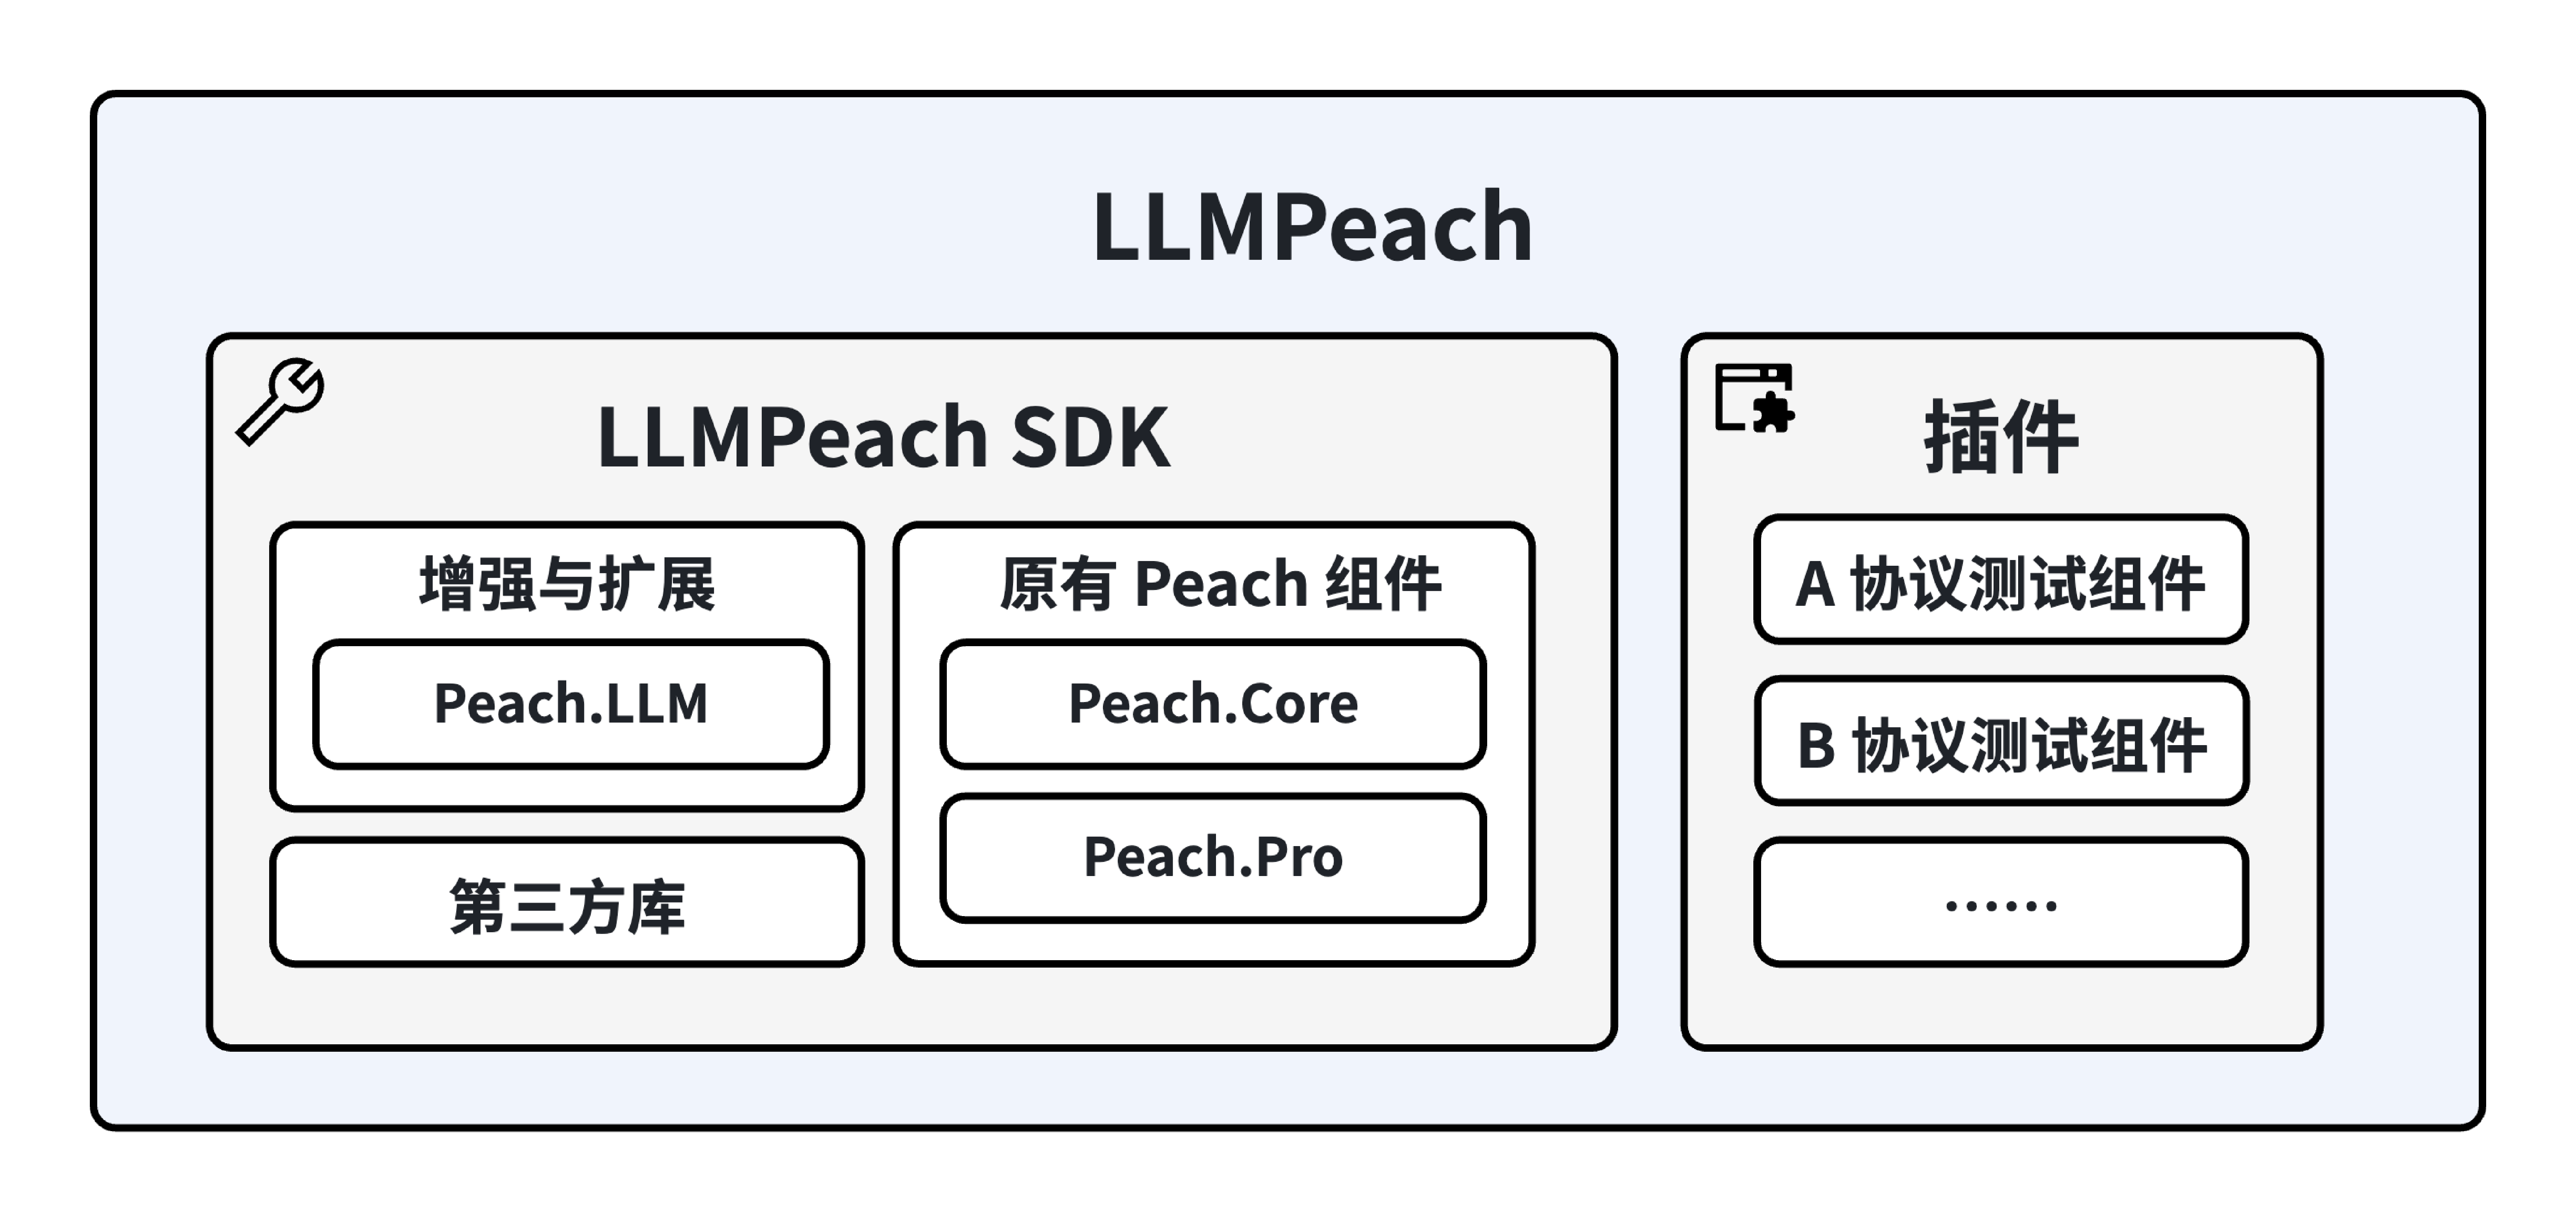
\includegraphics[width=0.8\textwidth]{source/llmpeach.pdf}
    \bicaption{LLMPeach 系统架构设计}{Architecture Design of LLMPeach}
    \label{fig:llmpeach_architecture}
\end{figure}

\subsection{Peach 框架的增强与扩展}

为了支持大语言模型生成的变异器和修复器，LLMPeach 对 Peach 框架进行了多方面的增强与扩展。

\textbf{Optional数据类型}。首先，在 Peach 的数据模型层面，LLMPeach 引入了 Optioal 数据类型，以弥补 Peach 原有数据模型在表达协议中可选字段时的不足。具体而言，Optional 作为一种条件数据容器，用于根据给定条件动态决定其内部字段是否参与解析与生成。

该类型通过两个核心属性实现语义控制：一是 src，用于指定参考字段路径；二是 expression，用于定义基于参考字段取值的逻辑表达式。在运行时，系统首先解析 src 指向的字段，并将其值绑定为表达式中的变量 value，随后对 expression 进行求值。当表达式结果为真时，Optional 内部的子元素将被正常解析与参与数据生成；否则，该结构将被跳过，从而实现对协议中条件字段的精确建模。

在数据解析（cracking）阶段，Optional 类型会在处理前动态评估条件表达式，仅在条件满足时才对子元素进行递归解析；否则直接跳过对应数据片段，从而避免无效解析带来的错误传播。在数据生成阶段，Optional 同样依据条件结果决定是否输出对应字段，若条件不满足，则生成空值或零长度数据，以保持整体数据结构的一致性。

图 \ref{fig:optional_example} 展示了一个 Optional 数据类型的使用示例。 在该示例中，will\_optional 作为一个 Optional 元素，其解析与生成完全依赖于 connect\_flags 字段的特定位（bit 2）的值。当该位被置为1时，will\_optional 内部的 will\_props、will\_topic 和 will\_payload 等字段将被正常处理；反之，则整个 will\_optional 结构将被跳过，从而实现了对 MQTT 协议中遗嘱消息相关字段的条件建模。

\begin{figure}[H]
\centering
\begin{lstlisting}[numbers=left, frame=single, breaklines=true, basicstyle=\codefont\small, frameround=tttt,rulecolor=\color{black},backgroundcolor=\color{white},belowskip=0pt,numberstyle=\small\color{gray}]
<DataModel name="mqtt_connect_payload_t">
    <Block name="client_id" ref="MQTT_String"/>

    <!-- Will Flag (bit 2) -->
    <Optional name="will_optional" src="variable_header.connect_flags" expression="(value &amp; 0x04) != 0">
      <Block name="will_props" ref="mqtt_properties_t"/>
      <Block name="will_topic" ref="MQTT_String"/>
      <Block name="will_payload" ref="MQTT_BinaryData"/>
    </Optional>

    <!-- Other fields... -->
</DataModel>
\end{lstlisting}
\bicaption{Optional 数据类型示例}{Example of Optional DataElement}
\label{fig:optional_example}
\end{figure}

\textbf{大模型变异器与修复器基类}。为了规范大语言模型生成的变异器和修复器的接口与行为，LLMPeach 在 SDK 中定义了 LLMMutator 和 LLMFixer 两个抽象基类。这些基类继承自 Peach 框架中相应的 Mutator 和 Fixer 基类，并在此基础上增加了针对大模型生成组件的特定接口要求和功能约束。

\textbf{测试组件检验器}。为了确保大语言模型生成的变异器和修复器能够正确编译并符合 Peach 的接口规范，LLMPeach 实现了一套自动化的测试组件检验器。该检验器实现了前文设计的变异器和修复器的检验流程，并将其提供给大模型智能体驱动的测试组件生成流水线使用。该检验器，能够在生成阶段后运行验证测试，并根据测试结果提供详细的错误报告，反馈给生成流水线，从而引导模型进行针对性的修正。

\textbf{两阶段变异策略实现}。LLMPeach 模糊测试框架按照Peach 的策略规范实现了前文设计的两阶段变异策略。